\documentclass[11pt,a4paper]{article}

% ---------- Sprache & Encoding ----------
\usepackage[utf8]{inputenc}
\usepackage[T1]{fontenc}
\usepackage{lmodern}

% ---------- Layout ----------
\usepackage[a4paper,margin=2.3cm]{geometry}
\usepackage{enumitem}
\usepackage{booktabs}
\usepackage{array}
\usepackage{tabularx}
\usepackage{graphicx}
\usepackage{import}
\usepackage{amsmath,amssymb}
\usepackage{xcolor}
\usepackage{tcolorbox}
\tcbuselibrary{skins,breakable}
\usepackage{fancyhdr}
\usepackage[hidelinks]{hyperref}
\usepackage{titlesec}
\usepackage{tikz}
\usepackage{needspace}

% ---------- Farben ----------
\definecolor{kfrblue}{HTML}{1F5C99}
\definecolor{warnorange}{HTML}{B45309}
\definecolor{warnbg}{HTML}{FFF3E0}
\definecolor{tipbg}{HTML}{EAF3EA}
\definecolor{tipgreen}{HTML}{2E7D32}

% ---------- Überschriften ----------
\titleformat{\section}{\large\bfseries\color{kfrblue}}{\thesection}{0.6em}{}
\titleformat{\subsection}{\normalsize\bfseries\color{kfrblue}}{\thesubsection}{0.6em}{}

% ---------- Kopf-/Fusszeile ----------
\pagestyle{fancy}
\fancyhf{}
\renewcommand{\headrulewidth}{0.4pt}
\fancyhead[L]{\small Physik 5.\,Klasse, Praktikum 08}
\fancyhead[R]{\small Anleitung}
\fancyfoot[C]{\small\thepage}

% ---------- Boxen ----------
\newtcolorbox{achtungbox}[1][]{%
  colback=warnbg, colframe=warnorange, coltitle=white, colbacktitle=warnorange,
  boxrule=0.8pt, arc=2pt,
  left=6pt, right=6pt, top=4pt, bottom=4pt, breakable,
  title={\textbf{Achtung: darauf kommt es an}#1},
  fonttitle=\small, fontupper=\small
}
\newtcolorbox{aufgabebox}[1][]{%
  colback=gray!6, colframe=kfrblue, coltitle=white, colbacktitle=kfrblue,
  boxrule=0.8pt, arc=2pt,
  left=6pt, right=6pt, top=4pt, bottom=4pt, breakable,
  title={\textbf{Aufgabe}#1}, fonttitle=\small, fontupper=\small
}
\newtcolorbox{loesungbox}[1][]{%
  colback=tipbg, colframe=tipgreen, coltitle=white, colbacktitle=tipgreen,
  boxrule=0.8pt, arc=2pt,
  left=6pt, right=6pt, top=4pt, bottom=4pt, breakable,
  title={\textbf{Musterlösung}#1}, fonttitle=\small, fontupper=\small
}

\setlist[itemize]{leftmargin=1.4em, itemsep=2pt, topsep=3pt}
\setlist[enumerate]{leftmargin=1.6em, itemsep=2pt, topsep=3pt}

% ---------- einfache Einheiten-Makros (kein siunitx nötig) ----------
\newcommand{\SI}[2]{#1\,#2}
\newcommand{\milli}{m}
\newcommand{\meter}{m}

% ---------- Lösungen ein-/ausblenden --------------------------------------
% Schülerexemplar (Standard): \solutionsfalse
% Lehrer-/Musterlösungsexemplar: \solutionstrue
\newif\ifsolutions
\solutionsfalse
% \solutionstrue

% ---------- Platz für Antworten (kariert) ---------------------------------
\newlength{\gridwidth}
\newcommand{\antwortraum}[1]{%
  \par\vspace{4pt}\noindent
  \setlength{\gridwidth}{\linewidth}%
  \begin{tikzpicture}
    \useasboundingbox (0,0) rectangle (\gridwidth,#1);
    \draw[step=0.5cm, gray!25, very thin] (0,0) grid (\gridwidth,#1);
    \draw[black, thin] (0,0) rectangle (\gridwidth,#1);
  \end{tikzpicture}
  \vspace{4pt}
}
\newcommand{\antwortraumS}{\antwortraum{2.5cm}}
\newcommand{\antwortraumM}{\antwortraum{4.5cm}}
\newcommand{\antwortraumL}{\antwortraum{8cm}}

% ---------- Freier Zeichenraum (Mindmap etc.) -----------------------------
\newcommand{\zeichenraum}[1][4.5cm]{%
  \par\vspace{4pt}\noindent
  \fbox{\begin{minipage}[t][#1][t]{\dimexpr\linewidth-2\fboxsep-2\fboxrule}\ \end{minipage}}
  \vspace{4pt}
}

% ---------- Feines Diagrammgitter (von Hand plotten) ----------------------
\newcommand{\diagrammraum}[1][10cm]{%
  \par\vspace{4pt}\noindent
  \setlength{\gridwidth}{\linewidth}%
  \begin{tikzpicture}
    \useasboundingbox (0,0) rectangle (\gridwidth,#1);
    \draw[step=0.2cm, gray!20, very thin] (0,0) grid (\gridwidth,#1);
    \draw[step=1cm, gray!55, thin] (0,0) grid (\gridwidth,#1);
    \draw[black, thin] (0,0) rectangle (\gridwidth,#1);
  \end{tikzpicture}
  \vspace{4pt}
}

\begin{document}
\thispagestyle{empty}

% ---------- Titelblock ----------
\begin{center}
  {\color{kfrblue}\Large\bfseries Praktikum 08: Linsenabbildung an der Sammellinse}\\[2pt]
  {\normalsize Kantonsschule Freudenberg, Physik 5.\ Klasse}
\end{center}
\vspace{4pt}
\noindent
\begin{tabularx}{\linewidth}{@{}X X@{}}
  Name/n: \dotfill & Gruppe: \dotfill \\
\end{tabularx}
\vspace{10pt}\hrule\vspace{10pt}

% ======================================================
\section{Lernziele}

Nach diesem Praktikum können Sie...
\begin{itemize}[nosep]
  \item die Abbildungsgleichung $\frac{1}{g}+\frac{1}{b}=\frac{1}{f}$ und den
    Abbildungsmassstab $\frac{B}{G}=\frac{b}{g}$ an einer Sammellinse experimentell
    überprüfen.
  \item die Grössen $g$, $b$, $G$ und $B$ an einem optischen Baukasten
    sauber messen und dabei eigene Messunsicherheiten begründet
    abschätzen.
  \item mithilfe der Fehlerrechnung eine Aussage zur Sicherheit eines
    gefundenen physikalischen Zusammenhangs machen.
  \item erklären, weshalb bei sehr kleiner Gegenstandsweite kein reelles Bild
    mehr auf der Mattscheibe erscheint.
\end{itemize}

\noindent\emph{Hinweis:} Die optischen Grundlagen (Hauptstrahlen,
Abbildungsgleichung, Abbildungsmassstab, Spezialfälle) sind im separaten
\textbf{Theorieskript zu Praktikum~08} zusammengestellt. Lesen Sie es vor
diesem Praktikum, insbesondere die Abschnitte~2 bis~6.

% ======================================================
\section{Material (pro Gruppe)}

\begin{itemize}[nosep]
  \item Pasco Optikbaukasten: Lichtquelle mit Pfeilkreuzobjekt, Sammellinse
    $f=\SI{75}{\milli\meter}$ (\emph{75\,mm FOCAL LENGTH -- CONVEX LENS}) im
    Halter, Mattscheibe, optische Schiene mit Massstab
  \item Verlängerungskabel
  \item Backpapier
  \item Tiefenmass
\end{itemize}

\begin{achtungbox}
\begin{itemize}[nosep]
  \item Die Lichtquelle kann nach längerem Betrieb warm werden: vorsichtig
    anfassen, insbesondere am Lampengehäuse.
  \item Nicht direkt in die eingeschaltete Lichtquelle blicken.
  \item Die Linse besteht aus Glas: an den Rändern anfassen, nicht auf die
    optische Fläche greifen, nicht fallen lassen.
\end{itemize}
\end{achtungbox}

% ======================================================
\section{Einbettung in bekanntes Wissen}

\begin{aufgabebox}
Zeichnen Sie ein Mindmap mit den Begriffen, die Ihnen zum Thema Brechung und
Sammellinsen noch geläufig sind (z.\,B.\ aus Praktikum~09 oder dem
Theorieskript).
\end{aufgabebox}
\zeichenraum[4.5cm]

% ======================================================
\section{Planung (im Plenum, vor dem Aufbau)}

\noindent Bevor Sie in der Gruppe zu messen beginnen, wird im Plenum
besprochen:

\begin{aufgabebox}
Diskutieren Sie gemeinsam:
\begin{itemize}[nosep]
  \item Wie stellen Sie die Lichtquelle auf der optischen Schiene auf,
    damit Sie alle folgenden Messungen mit demselben Aufbau durchführen
    können, ohne die Lichtquelle zu verschieben?
  \item Beim direkten Blick auf die Mattscheibe bildet sich manchmal nicht
    das Pfeilkreuz, sondern der Glühwendel der Lampe scharf ab. Wie liesse
    sich das mit dem Backpapier verhindern?
  \item Wie bestimmen Sie mit dem Tiefenmass die genaue Position der
    Linsenebene im Halter, statt nur die Aussenkante des Halters
    abzulesen?
  \item Was erwarten Sie laut Theorieskript (Abschnitt~6), sobald $g$
    kleiner als die Brennweite $f=\SI{75}{\milli\meter}$ wird? Woran
    könnten Sie das beim Messen erkennen?
\end{itemize}
\end{aufgabebox}
\antwortraumM

% ======================================================
\section{Vorbereitungsaufgabe: Bildkonstruktion von Hand}

\begin{aufgabebox}
Konstruieren Sie mit den drei Hauptstrahlen aus dem Theorieskript
(Abschnitt~2) das Bild des eingezeichneten Pfeils. Die Gegenstandsweite
liegt zwischen $f$ und $2f$ (vgl.\ Fall~3 im Theorieskript, Abschnitt~6).

\begin{center}
  \def\svgwidth{0.8\linewidth}
  \import{Bilder/}{bildkonstruktion_aufgabe.pdf_tex}
\end{center}
\end{aufgabebox}

\ifsolutions
\begin{loesungbox}
\begin{center}
  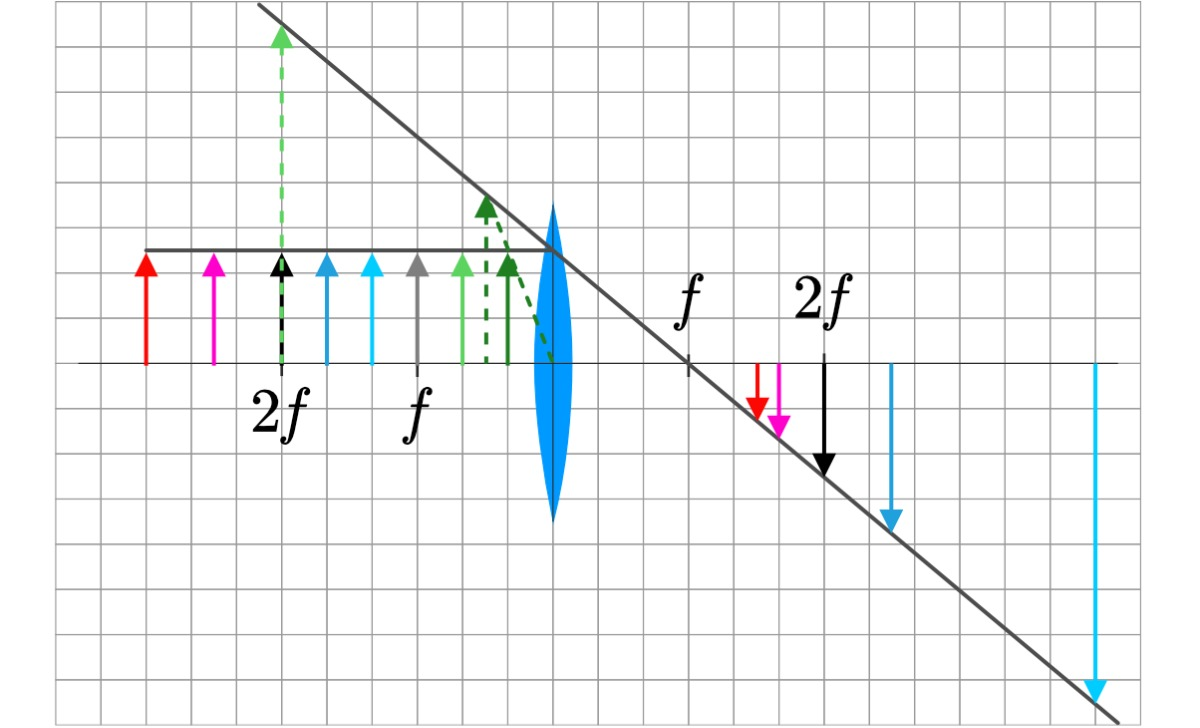
\includegraphics[width=0.85\linewidth]{Bilder/bildkonstruktion_bei_einer_sammellinse-aufgabe_Loesung.jpg}
\end{center}
\end{loesungbox}
\fi

% ======================================================
\section{Durchführung}

\begin{enumerate}[nosep]
  \item Bauen Sie die Lichtquelle, den Linsenhalter mit der
    $\SI{75}{\milli\meter}$-Linse und die Mattscheibe gemäss Skizze auf der
    optischen Schiene auf. Stellen Sie die Lichtquelle gemäss Ihrer
    Planung leicht überstehend auf, damit sie für alle folgenden Messungen
    an derselben Stelle bleiben kann.
  \item Legen Sie bei Bedarf ein Stück Backpapier zwischen Lichtquelle und
    Pfeilkreuz, damit dieses diffus beleuchtet wird.
  \item Bestimmen Sie mit dem Tiefenmass die genaue Lage der Linsenebene im
    Halter und lesen Sie daran die Gegenstandsweite $g$ auf der Schiene ab.
  \item Messen Sie die Gegenstandsgrösse $G$ direkt am Pfeilkreuz (sie
    bleibt für alle Messungen konstant).
  \item Stellen Sie für jeden Wert von $g$ in Tabelle~2 die Mattscheibe so
    ein, dass das Bild möglichst scharf erscheint, und lesen Sie die
    Bildweite $b$ sowie die Bildgrösse $B$ auf der Massstabsskala der
    Mattscheibe ab.
  \item Bestimmen Sie Ihre Messunsicherheit $\Delta b$ nur \emph{einmal},
    nicht pro Zeile: Verschieben Sie die Mattscheibe bei einer mittleren
    Gegenstandsweite ausgehend von der schärfsten Position so weit, bis
    Sie eine merkliche Unschärfe erkennen. Die halbe Breite dieses
    Bereichs ist Ihr $\Delta b$. Dieser Wert gilt für alle Zeilen.
  \item $g$, $B$ und $G$ messen Sie ebenfalls an einer Skala
    (Schienenmassstab bzw.\ Mattscheibenskala). Auch diese Ablesungen
    sind nicht exakt. Schätzen Sie $\Delta g$, $\Delta B$ und
    $\Delta G$ ebenfalls je \emph{einmal}: Wie fein können Sie dort
    wirklich noch ablesen? Tragen Sie $G$ und alle vier
    Messunsicherheiten in Tabelle~1 ein.
  \item Führen Sie alle Messungen zuerst für alle Werte von $g$ durch,
    bevor Sie mit den Berechnungen in Tabelle~2 beginnen.
\end{enumerate}

\begin{center}
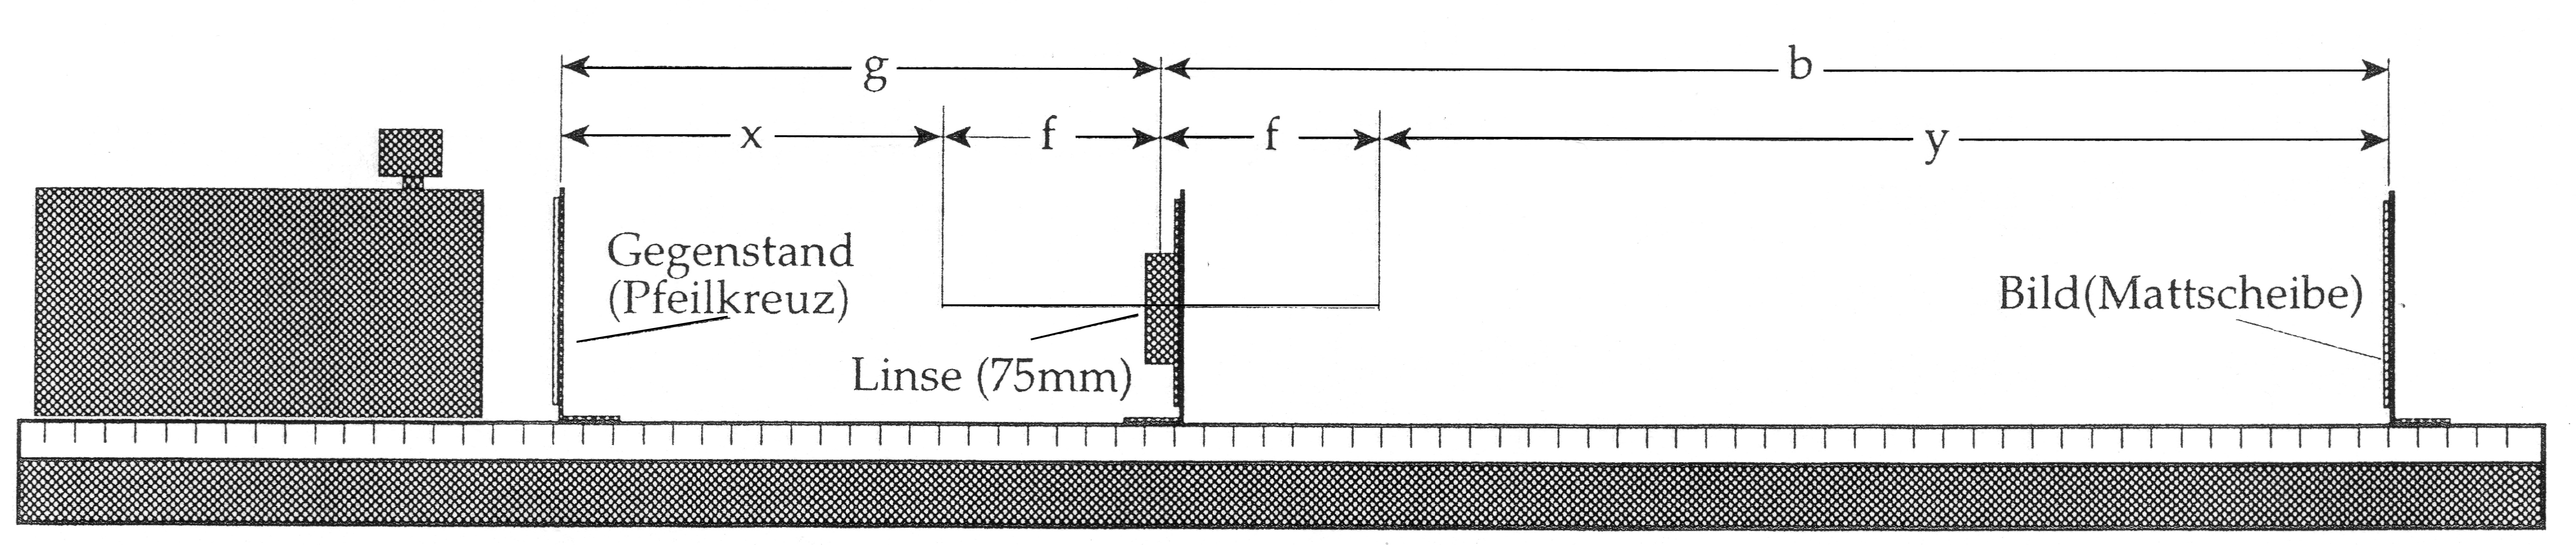
\includegraphics[width=\linewidth]{Bilder/Versuchsaufbau.jpg}
\end{center}

\vspace{0.8em}
\noindent\textbf{Tabelle 1: Gegenstandsgrösse und Messunsicherheiten}
\emph{(je einmal geschätzt, gelten für alle Zeilen von Tabelle~2)}

\begin{center}
\renewcommand{\arraystretch}{2.2}
\begin{tabularx}{\linewidth}{|>{\centering\arraybackslash}X|>{\centering\arraybackslash}X|>{\centering\arraybackslash}X|>{\centering\arraybackslash}X|>{\centering\arraybackslash}X|}
  \hline
  $G$ [mm] & $\Delta g$ [mm] & $\Delta b$ [mm] & $\Delta B$ [mm] & $\Delta G$ [mm] \\
  \hline
   & & & & \\
  \hline
\end{tabularx}
\end{center}

\noindent\textbf{Tabelle 2: Messwerte und Berechnungen}

\begin{center}
\renewcommand{\arraystretch}{2.4}
\begin{tabularx}{\linewidth}{|>{\centering\arraybackslash}X|>{\centering\arraybackslash}X|>{\centering\arraybackslash}X|>{\centering\arraybackslash}X|>{\centering\arraybackslash}X|>{\centering\arraybackslash}X|}
  \hline
  \multicolumn{3}{|c|}{\textbf{Messungen}} & \multicolumn{3}{c|}{\textbf{Berechnungen}} \\
  \hline
  $g$ [mm] & $b$ [mm] & $B$ [mm] & $\frac{1}{g}+\frac{1}{b}$ [mm$^{-1}$] & $\frac{B}{G}$ & $\frac{b}{g}$ \\
  \hline
  500 & & & & & \\
  \hline
  450 & & & & & \\
  \hline
  400 & & & & & \\
  \hline
  350 & & & & & \\
  \hline
  300 & & & & & \\
  \hline
  250 & & & & & \\
  \hline
  200 & & & & & \\
  \hline
  150 & & & & & \\
  \hline
  100 & & & & & \\
  \hline
  75 & \multicolumn{5}{l|}{\emph{siehe Aufgabe unten}} \\
  \hline
  50 & \multicolumn{5}{l|}{\emph{siehe Aufgabe unten}} \\
  \hline
\end{tabularx}
\end{center}

\begin{aufgabebox}
Bei $g=\SI{75}{\milli\meter}$ und $g=\SI{50}{\milli\meter}$ lässt sich kein
scharfes Bild mehr auf der Mattscheibe finden. Erklären Sie mithilfe des
Theorieskripts (Abschnitt~6), woran das liegt, und was Sie stattdessen
beobachten, wenn Sie direkt durch die Linse blicken.
\end{aufgabebox}
\antwortraumS

\ifsolutions
\begin{loesungbox}
Bei $g=\SI{75}{\milli\meter}=f$ liegt der Gegenstand genau im Brennpunkt
$F_2$: Parallelstrahl und Brennpunktstrahl verlassen die Linse parallel
zueinander und schneiden sich nie, es entsteht kein Bild. Bei
$g=\SI{50}{\milli\meter}<f$ liegt ein virtuelles Bild vor (Fall~4): Die
gebrochenen Strahlen schneiden sich nicht mehr hinter der Linse, nur ihre
rückwärtigen Verlängerungen vor der Linse. Ein solches Bild lässt sich
nicht auf einer Mattscheibe auffangen, ist aber sichtbar, wenn man direkt
durch die Linse blickt. Es erscheint dabei aufrecht und vergrössert.
\end{loesungbox}
\fi

% ======================================================
\section{Auswertung}

\begin{aufgabebox}
Weshalb untersuchen wir zur Überprüfung der Abbildungsgleichung nicht das
Abbildungsverhalten bei virtuellen Bildern (also $g<f$)?
\end{aufgabebox}
\antwortraumS

\ifsolutions
\begin{loesungbox}
Ein virtuelles Bild entsteht nicht durch tatsächlich konvergierende
Lichtstrahlen und lässt sich deshalb nicht auf der Mattscheibe auffangen.
Ohne Mattscheibe lässt sich die Bildweite $b$ nicht direkt und
reproduzierbar messen, eine quantitative Überprüfung der
Abbildungsgleichung ist damit auf diesem Weg nicht möglich.
\end{loesungbox}
\fi

\subsection{Aussage 1: Abbildungsmassstab}

\begin{aufgabebox}[: Berechnung]
Berechnen Sie für jede Zeile $B/G$ und $b/g$ aus Tabelle~2 (bereits
eingetragen). Bilden Sie für beide Spalten je den Mittelwert über alle
Zeilen und vergleichen Sie die beiden Mittelwerte: Stimmen sie überein?
\end{aufgabebox}
\antwortraumL

\begin{aufgabebox}[: Grafische Kontrolle]
Der Abbildungsmassstab $\frac BG=\frac bg$ lässt sich als Gerade
$y=m\cdot x+c$ auftragen. Definieren Sie selbst: Was tragen Sie bei sich
auf der $x$-Achse auf, was auf der $y$-Achse? Was müssten Steigung $m$ und
Achsenabschnitt $c$ betragen, wenn der Abbildungsmassstab stimmt?
\antwortraum{2cm}

Tragen Sie Ihre neun Wertepaare ins Diagramm ein und zeichnen Sie von Hand
die beste Gerade durch die Punkte. Lesen Sie Steigung und Achsenabschnitt
so genau wie möglich ab und vergleichen Sie sie mit Ihrer Erwartung.
\diagrammraum
Abgelesen: $m = $ \makebox[2.5cm]{\hrulefill} \hfill $c = $ \makebox[2.5cm]{\hrulefill}
\end{aufgabebox}

\begin{aufgabebox}[: Fehlerfortpflanzung]
Berechnen Sie für jede Zeile von Tabelle~2 die Differenz
$d=\dfrac bg-\dfrac BG$ (sollte laut Theorie $0$ sein) sowie ihren Fehler
(mit $\Delta b$, $\Delta g$, $\Delta B$, $\Delta G$ aus Tabelle~1;
Theorieskript, Abschnitt~7.3)
\[
  \Delta d = \frac bg\left(\frac{\Delta b}{b}+\frac{\Delta g}{g}\right)+\frac BG\left(\frac{\Delta B}{B}+\frac{\Delta G}{G}\right).
\]
Bilden Sie den Mittelwert $\bar d$ sowie
$\Delta\bar d=\frac1N\sqrt{\sum_i(\Delta d_i)^2}$ ($N$ = Anzahl
verwendeter Zeilen).
\end{aufgabebox}
\antwortraumL

\begin{aufgabebox}[: Aussagesicherheit]
Liegt $0$ innerhalb von $\bar d\pm\Delta\bar d$? Diskutieren Sie, was das
über die Sicherheit des Abbildungsmassstabs als physikalischen
Zusammenhang aussagt.
\end{aufgabebox}
\antwortraumM

\subsection{Aussage 2: Linsengleichung}

\begin{aufgabebox}[: Berechnung]
Bilden Sie den Mittelwert Ihrer Werte für $\frac{1}{g}+\frac{1}{b}$ aus
Tabelle~2. Berechnen Sie daraus die experimentell bestimmte Brennweite
\[
  f_{\text{exp}} = \frac{1}{\overline{\left(\tfrac1g+\tfrac1b\right)}}
\]
und vergleichen Sie sie mit dem Literaturwert $f=\SI{75}{\milli\meter}$
der verwendeten Linse.
\end{aufgabebox}
\antwortraumL

\begin{aufgabebox}[: Grafische Kontrolle]
Die Abbildungsgleichung $\frac1g+\frac1b=\frac1f$ lässt sich umstellen zu
$\frac1b=-\frac1g+\frac1f$, also als Gerade $y=m\cdot x+c$. Definieren Sie
selbst: Was tragen Sie bei sich auf der $x$-Achse auf, was auf der
$y$-Achse? Was bedeuten Steigung $m$ und Achsenabschnitt $c$ physikalisch,
und welche Werte erwarten Sie dafür?
\antwortraum{2cm}

Tragen Sie Ihre neun Wertepaare ins Diagramm ein und zeichnen Sie von Hand
die beste Gerade durch die Punkte. Lesen Sie Steigung und Achsenabschnitt
ab und bestimmen Sie daraus $f$. Passt die abgelesene Steigung zu Ihrer
Erwartung?
\diagrammraum
Abgelesen: $m = $ \makebox[2.5cm]{\hrulefill} \hfill $c = $ \makebox[2.5cm]{\hrulefill} \hfill $f = $ \makebox[2.5cm]{\hrulefill}
\end{aufgabebox}

\begin{aufgabebox}[: Fehlerfortpflanzung]
Berechnen Sie für jede Zeile von Tabelle~2 die Fehler
$\Delta(1/g)=\Delta g/g^2$ und $\Delta(1/b)=\Delta b/b^2$ sowie deren
Summe (mit $\Delta g$, $\Delta b$ aus Tabelle~1; Theorieskript,
Abschnitt~7.2). Bestimmen Sie daraus den Fehler des Mittelwerts von
$\frac{1}{g}+\frac{1}{b}$ über
\[
  \Delta\overline{\left(\tfrac1g+\tfrac1b\right)}=\frac1N\sqrt{\sum_i\left(\Delta(1/g)_i+\Delta(1/b)_i\right)^2}
\]
($N$ = Anzahl verwendeter Zeilen) und geben Sie damit $f_{\text{exp}}$
mitsamt Unsicherheit an.
\end{aufgabebox}
\antwortraumL

\begin{aufgabebox}[: Aussagesicherheit]
Liegt der Literaturwert $f=\SI{75}{\milli\meter}$ innerhalb Ihres
Ergebnisses $f_{\text{exp}}\pm\Delta f_{\text{exp}}$? Diskutieren Sie, was
das über die Sicherheit der Abbildungsgleichung als physikalischen
Zusammenhang aussagt.
\end{aufgabebox}
\antwortraumM

% ======================================================
\section{Fehlerquellen (im Plenum)}

\begin{aufgabebox}
Sammeln Sie gemeinsam die wichtigsten Fehlerquellen dieses Versuchs und
ordnen Sie sie als zufällig oder systematisch ein.
\end{aufgabebox}
\antwortraumM

% ======================================================
\section{Mein Ergebnis}

\begin{aufgabebox}
Fassen Sie in ein bis zwei Sätzen zusammen: Wie gross ist Ihre
experimentell bestimmte Brennweite $f_{\text{exp}}\pm\Delta f_{\text{exp}}$,
und stimmt sie mit dem Literaturwert $\SI{75}{\milli\meter}$ überein?
\end{aufgabebox}
\antwortraumS

\end{document}
